\documentclass[crop,tikz]{standalone}

\usepackage[utf8]{inputenc}

% 'crop' is the default for v1.0, before it was 'preview'
%\usetikzlibrary{...}% tikz package already loaded by 'tikz' option
\usetikzlibrary{arrows} 

\newcommand{\periodGraph}[2]{
	\begin{scope}[shift={(#1*6,#2*6)}]
		\begin{scope}
			%draw graph period cell with some stuff going off boundary for effect
			\filldraw (-2,-1) circle (.1);
			\filldraw (0,-1) circle (.1);
			\filldraw (2,-1) circle (.1);
			\filldraw (0,{sqrt(10)-1}) circle (.1);
			
			%draw graph edges;
			%internal
			\draw[->>] (-2,-1) -- (-1,-1);					\draw (-1,-1) -- (0,-1);
			\draw[->>] (0,-1) -- (1,-1);					\draw (1,-1) -- (2,-1);
			\draw[->>] (-2,-1) -- (-1,{-1+0.5*sqrt(10)});	\draw (-1,{-1+0.5*sqrt(10)}) -- (0,{sqrt(10)-1});
			\draw[->>] (2,-1) -- (1,{-1+0.5*sqrt(10)});	\draw (1,{-1+0.5*sqrt(10)}) -- (0,{sqrt(10)-1});
			%cross-boundary
			\draw[->>] (0,{sqrt(10)-1}) -- (0,3);
			\draw (0,-3) -- (0,-1);
			\draw[->>] (2,-1) -- (3,-1);
			\draw (-3,-1) -- (-2,-1);
		\end{scope}
	\end{scope}
}

\begin{document}

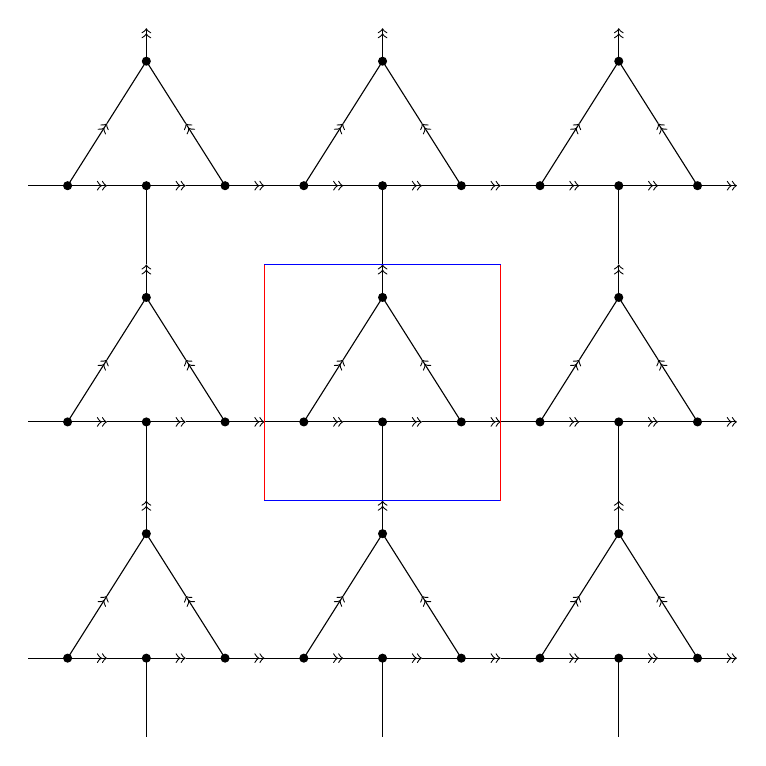
\begin{tikzpicture}	
	\begin{scope}[scale=1/2]
		%draw ``lattice" of period cells
		\foreach \x in {-1,...,1}{
			\foreach \y in {-1,...,1}{
				\periodGraph{\x}{\y}
			}
		}
		%unit cell boundary with colours for future direction-association
		\draw[red] (-3,-3) -- (-3,3);		\draw[blue] (-3,-3) -- (3,-3);
		\draw[red] (3,-3) -- (3,3);			\draw[blue] (-3,3) -- (3,3);

	\end{scope}
\end{tikzpicture}

\end{document}